
\section{Numerical Methods}

\begin{frame}{Approximation for stochastic differential equations}
	\begin{equation*}
	dX=\alpha(X)dt+{\color{red}\beta(X)dW}
	\end{equation*}
	\begin{center}
	$\alpha$, $\beta$ are functions of X.	
	\end{center}
	\begin{itemize}
		\item It's difficult to find an explicit solution.
		\item We can make simulations.
	\end{itemize}
\end{frame}

%\begin{frame}{It\^{o}'s Formulas}
\begin{frame}{Ito's Formulas}
  	\begin{itemize}
   		\item First version: $$f(B(b))-f(B(a))=\int_{a}^{b}{\frac{\partial f}{\partial B} 				dB}+\int_{a}^{b}{\frac{1}{2} \frac{\partial^2 f}{\partial B^2} dt} $$\\
    		\item Second version: $$f(b,B(b))-f(a,B(a))=\int_{a}^{b}{\frac{\partial f}{\partial B} 			dB}+\int_{a}^{b}{\left(\frac{\partial f}{\partial s}+\frac{1}{2}\frac{\partial^2 f}
    		{\partial B^2}\right) ds}$$\\
    		\item Third version: The Stochastic Chain Rule
    		$$\theta (t,x_t)=\theta(a,x_a)+\int_{a}^{t}\frac{\partial \theta}{\partial s}ds+
    		\int_{a}^{t}f\frac{\partial \theta}{\partial x}dW+
  		\int_{a}^{t}g\frac{\partial \theta}{\partial x}+f^2 \frac{1}{2} \frac{\partial ^2\theta}
  		{\partial x^2}ds$$\\
  	\end{itemize}
\end{frame}

\begin{frame}{Numerical methods}
Integral form of a SDE: 
$$X(t)=X_0+\int_{0}^{t}f(X(s))ds+{\color{red}\int_{0}^{t}g(X(s))dW(s)}$$

X(t) is a random variable for each value of t. To apply numerical methods:
	\begin{itemize}
		\item Discretized time steps	
		\item X(t) will be the limit as our stepsize goes to zero.
	\end{itemize}
\end{frame}

\begin{frame}{Euler-Maruyama method}
Let $\tau_j=j\Delta t$. In the in the interval [0,L] we have the EM method:\bigskip\\
$$X_j=X_{j-1}+f(X_{j-1})\Delta t+g(X_{j-1})(W(\tau_j)-W(\tau_{j-1}))$$
 which is an approximation for the equation
$$X(\tau_j)=X(\tau_{j-1})+\int_{\tau_{j-1}}^{\tau_{j}}f(X(s))ds+\int_
{\tau_{j-1}}^{\tau_{j}}X(s)dW(s)$$
%We have Euler's method in the deterministic case ($g\equiv 0$)
\end{frame}

\begin{frame}
\begin{block}{Strong Convergence}
We say that a method has strong order of convergence equal to $\gamma$ if there exists a constant C such that:
$$E|X_n-X(\tau)|\leq C \Delta t^\gamma$$
for any fixed $\tau=n \Delta t \in [0,T]$ and $\Delta t$ sufficiently small.
\end{block}
\bigskip
The EM method has strong order of convergence of $\gamma=\frac{1}{2}$.
\end{frame}

\begin{frame}{Milstein's method}
The Milstein method raises the strong order of convergence to 1:	
	\begin{equation*}
	\begin{split}
	X_{j} & =X_{j-1}+ f(X_{j-1}) \; \Delta t + g(X_{j-1})(W(\tau_j)-W(\tau_{j-1}))\\
	  &\quad +\frac{1}{2}g(X_{j-1})g'(X_{j-1})((W(\tau_j)-W(\tau_{j-1}))^2-\Delta t)
	\end{split}
	\end{equation*}
\end{frame}

\begin{frame}{Example}
If we consider the differential equation:
\begin{equation*}
  dX=\alpha X dt+ \beta X dW,
\end{equation*}
the theoretical solution is: 
\begin{equation*}
  X(t)=X_{0}\exp{\left((\alpha -\frac{1}{2}\beta ^2)t +\beta W(t)\right)}
\end{equation*}
\end{frame}

\begin{frame}
	\begin{center}
	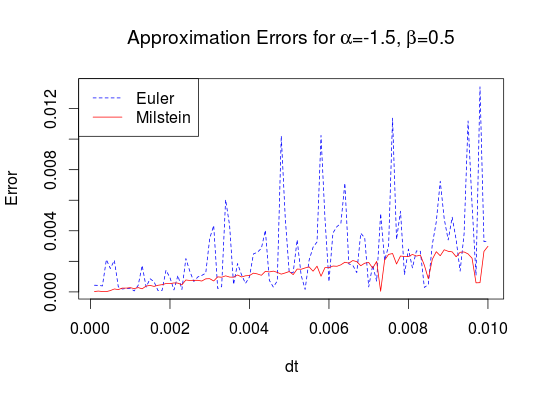
\includegraphics[scale=0.55]{alpham15_beta05.png} 
	\end{center}
\end{frame}

\begin{frame}
A system of equations can be expressed in differential form:
	\begin{eqnarray*}
		dx&=&f_1(x,y)dt+{\color{red}g_1(x,y)dW}\\
		dy&=&f_2(x,y)dt+{\color{red}g_2(x,y)dW}\\
	\end{eqnarray*}
The equivalent integral form is the following:
	\begin{eqnarray*}
		x_t=x_a+\int_{a}^{t}f_1 ds+{\color{red}\int_{a}^{t}g_1dW_1}\\
		y_t=y_a+\int_{a}^{t}f_2 ds+{\color{red}\int_{a}^{t}g_2dW_2}\\
	\end{eqnarray*}	
\end{frame}


\begin{frame}
Applying the chain rule for $f_1$:
	\begin{equation*}
	\begin{split}
	f_1(x_j,y_j) &=f_1(x_{j-1},y_{j-1})+f_{1x}(x_{j-1},y_{j-1})(x-x_{j-1})\\
	& \quad +f_{1y}(x_{j-1},y_{j-1})(y-y_{j-1})+\frac{1}{2} f_{1xx}(x_{j-1},y_{j-1})(x-
	x_{j-1})^2\\
	& \quad +f_{1xy}(x_{j-1},y_{j-1})(x-x_{j-1})(y-y_{j-1})+\\
	& \quad \frac{1}{2}f_{1yy}(x_{j-1},y_{j-1})(y-y_{j-1})^2
	\end{split}
	\end{equation*}
Substitute into the integral form:
	\begin{eqnarray*}
	x_j-x_{j-1} & \approx & \int_{\tau_{j-1}}^{\tau_{j}}f_1 ds+\int_{\tau_{j-1}}^{\tau_{j}}g_1dW_1
	\end{eqnarray*}
\end{frame}


\begin{frame}
%I need to fix how it looks
Similarly for $g_1$ and if we ignore the high order terms:
	\begin{equation*}
	\begin{split}
	x_{j} & \approx x_{j-1}+f_1(x_{j-1},y_{j-1})\Delta t+g_1(x_{j-1},y_{j-1})\Delta W_1\\
	& \quad +g_{1x}(x_{j-1},y_{j-1})\int_{\tau_{j-1}}^{\tau_{j}}
	\int_{\tau_{j-1}}^{s}g_1dW_1dW_1\\
	& \quad	+g_{1y}(x_{j-1},y_{j-1})\int_{\tau_{j-1}}^{\tau_{j}}\int_{\tau_{j-1}}^{t}
	g_2dW_2dW_1\\
	\end{split}
	\end{equation*}	
\end{frame}


\begin{frame}
Applying the chain rule again:
	\begin{equation*}
	\begin{split}
	x_{j} &= x_{j-1}+f_1(x_{j-1},y_{j-1})\Delta t+g_1(x_{j-1},y_{j-1})\Delta W_1\\
	&\quad +\frac{1}{2}g_{1x}(x_{j-1},y_{j-1})g_{1}(x_{j-1},y_{j-1})(\Delta W_1^2-\Delta t)\\
	&\quad +g_{1y}(x_{j-1},y_{j-1})g_2(x_{j-1},y_{j-1})\Delta W_1 \Delta W_2\\
	\end{split}
	\end{equation*}
\end{frame}

\begin{frame}
Similarly:
\begin{equation*}
	\begin{split}
	y_{j}&=y_{j-1}+f_2(x_{j-1},y_{j-1})\Delta t+g_2(x_{j-1},y_{j-1})\Delta W_2\\
	&\quad +\frac{1}{2}g_{2x}(x_{j-1},y_{j-1})g_{1}(x_{j-1},y_{j-1})\Delta W_1 \Delta W_2\\
	&\quad +g_{2y}(x_{j-1},y_{j-1})g_2(x_{j-1},y_{j-1})(\Delta W_2^2-\Delta t)\\
	\end{split}
	\end{equation*}
\end{frame}




